\documentclass[12pt,a4paper]{article}

\usepackage[utf8]{inputenc}
\usepackage[T1]{fontenc}
\usepackage[french]{babel}
\usepackage{geometry}
\usepackage{graphicx}
\usepackage{xcolor}
\usepackage{float}
\usepackage{array}
\usepackage{booktabs}
\usepackage{hyperref}
\usepackage{listings}
\usepackage{caption}
\usepackage{amsmath}
\usepackage{amssymb}
\usepackage{enumitem}
\usepackage{setspace}
\usepackage{fancyhdr}
\usepackage{titlesec}

\geometry{margin=2cm}
\setstretch{1.0}
\setlength{\headheight}{15pt}

\hypersetup{
    colorlinks=true,
    linkcolor=projectnavy,
    urlcolor=projectblue,
    citecolor=projectnavy
}

\definecolor{codegray}{RGB}{245,245,245}
\definecolor{codeblue}{RGB}{40,70,120}
\definecolor{projectblue}{RGB}{28,93,170}
\definecolor{projectnavy}{RGB}{18,44,76}
\definecolor{projectorange}{RGB}{245,179,36}
\definecolor{projectred}{RGB}{219,62,78}
\definecolor{softgray}{RGB}{248,249,251}

\lstdefinestyle{pythonstyle}{
    language=Python,
    backgroundcolor=\color{codegray},
    basicstyle=\ttfamily\scriptsize,
    keywordstyle=\color{codeblue}\bfseries,
    commentstyle=\color{gray},
    stringstyle=\color{teal},
    showstringspaces=false,
    breaklines=true,
    frame=single,
    rulecolor=\color{gray},
    columns=fullflexible
}

\pagestyle{fancy}
\fancyhf{}
\lhead{Mini-projet IA}
\rhead{Puissance 4}
\cfoot{\thepage}

\titleformat{\section}{\Large\bfseries\color{projectnavy}}{\thesection}{0.8em}{}
\titleformat{\subsection}{\large\bfseries\color{projectblue}}{\thesubsection}{0.8em}{}

\newcommand{\screenshotplaceholder}[3]{
    \begin{figure}[H]
        \centering
        \IfFileExists{#1}{
            \includegraphics[width=#2\textwidth]{#1}
        }{
            \fbox{
                \begin{minipage}[c][6cm][c]{#2\textwidth}
                    \centering
                    \textbf{Emplacement capture d'écran}\\[0.4cm]
                    Ajouter l'image : \texttt{\detokenize{#1}}
                \end{minipage}
            }
        }
        \caption{#3}
    \end{figure}
}

\newcommand{\keyword}[1]{\textbf{\textcolor{projectnavy}{#1}}}

\begin{document}
\pagenumbering{gobble}

\begin{titlepage}
\centering
\vspace*{0.1cm}

\begin{minipage}{0.45\textwidth}
    \raggedright
    
\includegraphics[width=0.50\textwidth]{logos/logo.png}
\end{minipage}
\hfill
\begin{minipage}{0.45\textwidth}
    \raggedleft
    
\includegraphics[width=0.46\textwidth]{logos/ilia.jpeg}
\end{minipage}

\vspace{0.8cm}

{\Large \textbf{Université Moulay Ismaïl}}\\[0.2cm]
{\large Faculté des Sciences et Techniques Errachidia}\\[0.15cm]
{\large Cycle d'Ingénieur d'État}\\[0.15cm]
{\large Filière : \textbf{Ingénierie Logicielle et Intelligence Artificielle}}

\vspace{0.7cm}
\rule{0.9\textwidth}{1pt}
\vspace{0.7cm}

{\Large \textbf{Compte rendu de mini-projet}}\\[0.25cm]
{\Huge \textcolor{projectnavy}{\textbf{Intelligence Artificielle}}}

\vspace{0.8cm}

\fcolorbox{projectnavy}{gray!10}{
\begin{minipage}{0.86\textwidth}
\centering
\vspace{0.45cm}
{\Huge \textbf{\textcolor{projectnavy}{Puissance 4}}}\\[0.35cm]
{\Large \textcolor{projectblue}{Jeu de stratégie avec agent intelligent}}\\[0.25cm]
{\large Algorithme Min-Max avec élagage Alpha-Bêta}
\vspace{0.45cm}
\end{minipage}
}

\vspace{0.8cm}

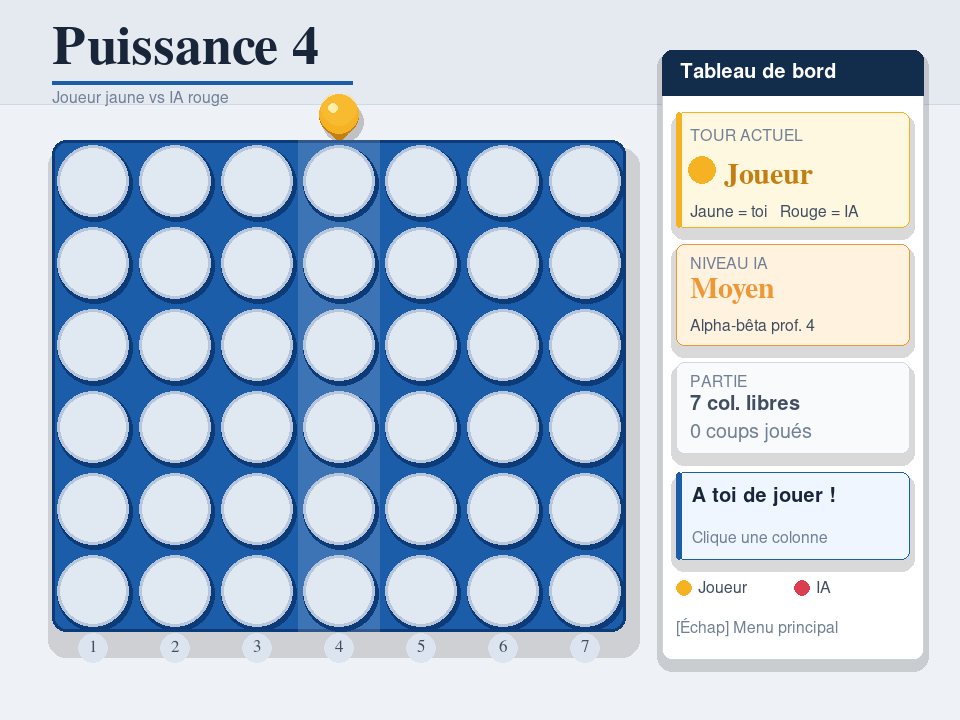
\includegraphics[width=0.58\textwidth]{screenshots/interface_accueil.png}

\vfill

\begin{minipage}{0.45\textwidth}
\raggedright
\textbf{\large Réalisé par :}\\[0.3cm]
Laghrib Salim\\
Zouhri Salma
\end{minipage}
\hfill
\begin{minipage}{0.45\textwidth}
\raggedleft
\textbf{\large Encadré par :}\\[0.3cm]
Pr. Khaddouj Taifi
\end{minipage}

\vspace{0.7cm}
\rule{0.9\textwidth}{1pt}
\vspace{0.3cm}
{\large \textbf{Année universitaire : 2025--2026}}
\end{titlepage}

\pagenumbering{roman}
\section*{Résumé}

Ce compte rendu présente la conception et la réalisation d'un jeu de stratégie \keyword{Puissance 4} intégrant un agent intelligent. Le projet répond au cahier des charges du mini-projet d'intelligence artificielle : présenter la méthode utilisée, étudier sa complexité, implémenter l'algorithme en langage Python et fournir une interface graphique valorisant l'application.

Le système développé permet à un joueur humain d'affronter une intelligence artificielle. L'agent choisit ses coups à partir de l'algorithme \keyword{Min-Max}, puis d'une version optimisée par \keyword{élagage alpha-bêta}. Comme l'arbre complet du Puissance 4 est trop grand pour être exploré entièrement, l'algorithme utilise une profondeur limitée et une fonction heuristique d'évaluation du plateau. Cette heuristique favorise les positions centrales, les alignements prometteurs et les coups qui bloquent les menaces adverses.

Le projet est structuré en modules : gestion du plateau, logique de l'IA, interface graphique et lancement de l'application. L'interface est réalisée avec \texttt{Pygame}, tandis que le plateau est représenté par une matrice \texttt{NumPy}. Les tests effectués montrent que l'IA sait gagner lorsqu'un coup immédiat est disponible, bloquer une menace directe et adapter son niveau de difficulté selon la profondeur de recherche.

\vspace{0.4cm}
\noindent\textbf{Mots-clés :} Intelligence artificielle, jeu de stratégie, Puissance 4, Min-Max, élagage alpha-bêta, heuristique, Python, Pygame.

\newpage
\tableofcontents
\newpage
\pagenumbering{arabic}

\section{Introduction et présentation de la méthode}

L'intelligence artificielle occupe une place importante dans les jeux de stratégie, car ces derniers offrent un cadre clair pour étudier la prise de décision, l'anticipation et l'optimisation. Dans ce mini-projet, nous avons choisi de réaliser un jeu de \keyword{Puissance 4} dans lequel un joueur humain affronte un agent intelligent.

Le Puissance 4 est un jeu à deux joueurs qui se déroule sur une grille de six lignes et sept colonnes. À chaque tour, un joueur choisit une colonne ; le jeton tombe alors automatiquement dans la case libre la plus basse de cette colonne. L'objectif est d'aligner quatre jetons identiques horizontalement, verticalement ou diagonalement avant l'adversaire.

Ce jeu est particulièrement adapté à l'étude de l'algorithme Min-Max. Chaque décision peut être représentée comme un arbre de possibilités : l'IA joue un coup, le joueur répond, puis l'IA rejoue, et ainsi de suite. L'agent intelligent doit donc anticiper les conséquences de ses actions tout en supposant que l'adversaire cherchera lui aussi à jouer de manière rationnelle.

Le travail réalisé respecte le plan demandé dans la consigne du mini-projet : une introduction avec présentation de la méthode, une étude de complexité, une implémentation de l'algorithme en Python pour résoudre un problème de jeu de stratégie, puis une conclusion. Le projet correspond à la catégorie \keyword{jeu de stratégie} et utilise l'algorithme \keyword{Min-Max} avec élagage alpha-bêta.

\subsection{Objectifs du projet}

Les objectifs principaux de ce mini-projet sont les suivants :

\begin{itemize}[leftmargin=1.2cm]
    \item modéliser correctement les règles du Puissance 4 ;
    \item représenter le plateau sous une forme exploitable par un programme ;
    \item implémenter un agent intelligent capable de choisir un coup pertinent ;
    \item étudier la complexité de la méthode utilisée ;
    \item proposer une interface graphique claire pour jouer contre l'IA ;
    \item tester le comportement de l'agent dans des situations de victoire et de blocage.
\end{itemize}

\subsection{Choix du mini-projet}

Dans la liste proposée pour le module, notre projet correspond à la catégorie \keyword{jeu de stratégie}. Nous avons retenu le Puissance 4 parce que ses règles sont simples à comprendre, mais sa résolution nécessite une vraie stratégie. Le jeu demande d'évaluer plusieurs coups à l'avance, d'identifier les menaces adverses et de contrôler les zones importantes du plateau.

\screenshotplaceholder{screenshots/interface_accueil.png}{0.66}{Interface d'accueil du jeu développé}


\subsection{Présentation générale du jeu}

\subsubsection{Règles du Puissance 4}

Le Puissance 4 se joue sur une grille de $6 \times 7$, soit 42 cases. Deux joueurs placent alternativement leurs jetons dans une colonne. En raison de la gravité, un jeton ne peut pas être placé n'importe où : il occupe automatiquement la position libre la plus basse de la colonne choisie.

Une partie se termine dans l'un des cas suivants :

\begin{itemize}[leftmargin=1.2cm]
    \item un joueur aligne quatre jetons de sa couleur ;
    \item le plateau est rempli sans alignement gagnant, ce qui produit un match nul.
\end{itemize}

Les alignements gagnants peuvent apparaître dans quatre directions : horizontale, verticale, diagonale montante ou diagonale descendante. La détection de ces alignements est donc une partie essentielle de la logique du jeu.

\subsubsection{Modélisation du problème}

Un état du jeu est défini par le contenu du plateau et par le joueur dont c'est le tour. Dans notre implémentation, chaque case du plateau prend l'une des trois valeurs suivantes :

\begin{table}[H]
    \centering
    \begin{tabular}{cl}
        \toprule
        Valeur & Signification \\
        \midrule
        \texttt{0} & Case vide \\
        \texttt{1} & Jeton du joueur humain \\
        \texttt{2} & Jeton de l'intelligence artificielle \\
        \bottomrule
    \end{tabular}
    \caption{Codage des cases du plateau}
\end{table}

Le choix d'une matrice est naturel, car il correspond directement à la structure de la grille. Il facilite également le parcours des lignes, colonnes et diagonales pour détecter les victoires et calculer le score heuristique.

\subsubsection{Contraintes du projet}

Selon la consigne fournie pour le mini-projet, le compte rendu doit inclure une introduction avec présentation de la méthode, une analyse de la complexité, une implémentation de l'algorithme dans un langage de programmation, ainsi qu'une conclusion. La réalisation d'une interface graphique est recommandée afin de valoriser l'application.

Notre projet répond à ces attentes de la manière suivante :

\begin{itemize}[leftmargin=1.2cm]
    \item une implémentation Python complète ;
    \item une interface graphique interactive avec \texttt{Pygame} ;
    \item une IA fondée sur \keyword{Min-Max} et l'élagage \keyword{alpha-bêta} ;
    \item une séparation claire entre logique du jeu, IA et affichage ;
    \item des captures d'écran montrant les principaux états de l'application.
\end{itemize}


\subsection{Méthode d'intelligence artificielle}

\subsubsection{Principe de l'algorithme Min-Max}

L'algorithme Min-Max est utilisé dans les jeux à deux joueurs, à somme nulle, dans lesquels l'amélioration de la situation d'un joueur correspond à la dégradation de la situation de l'autre. Dans notre projet, l'IA est le joueur maximisant, tandis que l'humain est considéré comme le joueur minimisant.

L'idée générale est la suivante : pour chaque coup possible de l'IA, le programme simule les réponses possibles du joueur, puis les coups suivants de l'IA, jusqu'à une profondeur limitée. Les feuilles de cet arbre sont évaluées par une fonction de score. L'IA choisit ensuite le coup qui maximise son résultat en supposant que l'adversaire jouera de façon optimale.

\begin{table}[H]
    \centering
    \begin{tabular}{p{4cm}p{9cm}}
        \toprule
        Élément & Rôle dans l'algorithme \\
        \midrule
        Nœud & État possible du plateau \\
        Branche & Coup possible dans une colonne valide \\
        Niveau max & Tour de l'IA, qui cherche le meilleur score \\
        Niveau min & Tour du joueur humain, qui cherche à réduire le score de l'IA \\
        Feuille & État terminal ou état atteint à la profondeur maximale \\
        \bottomrule
    \end{tabular}
    \caption{Interprétation de l'arbre de jeu}
\end{table}
\newpage
\subsubsection{Pseudo-code de Min-Max}

Le fonctionnement de Min-Max peut être résumé par le pseudo-code suivant :

\begin{lstlisting}[style=pythonstyle, caption={Pseudo-code simplifié de Min-Max}]
fonction minimax(plateau, profondeur, ia_joue):
    si plateau terminal ou profondeur = 0:
        retourner evaluation(plateau)

    si ia_joue:
        meilleur_score = -infini
        pour chaque colonne valide:
            simuler le coup de l'IA
            score = minimax(nouveau_plateau, profondeur - 1, faux)
            meilleur_score = max(meilleur_score, score)
        retourner meilleur_score

    sinon:
        meilleur_score = +infini
        pour chaque colonne valide:
            simuler le coup du joueur
            score = minimax(nouveau_plateau, profondeur - 1, vrai)
            meilleur_score = min(meilleur_score, score)
        retourner meilleur_score
\end{lstlisting}

\subsubsection{Limitation par profondeur}

Même si le Puissance 4 paraît simple, l'arbre de jeu devient rapidement très grand. Il n'est donc pas réaliste d'explorer toutes les parties jusqu'à la fin. Nous utilisons une profondeur limitée : lorsque cette profondeur est atteinte, l'algorithme ne connaît pas encore forcément le gagnant, mais il estime la qualité du plateau grâce à une heuristique.

Cette approche constitue un compromis entre qualité de décision et temps d'exécution. Une profondeur faible rend l'IA rapide, mais moins stratégique. Une profondeur élevée rend l'IA plus forte, mais augmente fortement le temps de calcul.


\subsection{Élagage alpha-bêta}

\subsubsection{Motivation}

Le Min-Max simple explore toutes les branches de l'arbre jusqu'à la profondeur fixée. Or certaines branches ne peuvent pas modifier la décision finale. L'élagage alpha-bêta permet d'éviter l'exploration de ces branches inutiles.

Cette optimisation ne change pas le résultat théorique de Min-Max : elle permet d'obtenir le même choix, mais en visitant moins d'états lorsque l'ordre d'exploration est favorable.

\subsubsection{Définition de alpha et bêta}

Deux bornes sont utilisées pendant la recherche :

\begin{itemize}[leftmargin=1.2cm]
    \item $\alpha$ représente le meilleur score déjà garanti pour le joueur maximisant, c'est-à-dire l'IA ;
    \item $\beta$ représente le meilleur score déjà garanti pour le joueur minimisant, c'est-à-dire le joueur humain.
\end{itemize}

Lorsque la condition $\alpha \geq \beta$ est vérifiée, l'algorithme peut arrêter l'exploration de la branche courante. En effet, le joueur rationnel ne choisira pas une branche qui mène à un résultat moins favorable que ce qu'il peut déjà garantir ailleurs.

\subsubsection{Pseudo-code de alpha-bêta}

\begin{lstlisting}[style=pythonstyle, caption={Pseudo-code de Min-Max avec élagage alpha-bêta}]
fonction alphabeta(plateau, profondeur, alpha, beta, ia_joue):
    si plateau terminal ou profondeur = 0:
        retourner evaluation(plateau)

    si ia_joue:
        valeur = -infini
        pour chaque colonne valide:
            simuler le coup de l'IA
            valeur = max(valeur, alphabeta(nouveau_plateau,
                                           profondeur - 1,
                                           alpha, beta, faux))
            alpha = max(alpha, valeur)
            si alpha >= beta:
                arreter la boucle
        retourner valeur

    sinon:
        valeur = +infini
        pour chaque colonne valide:
            simuler le coup du joueur
            valeur = min(valeur, alphabeta(nouveau_plateau,
                                           profondeur - 1,
                                           alpha, beta, vrai))
            beta = min(beta, valeur)
            si alpha >= beta:
                arreter la boucle
        retourner valeur
\end{lstlisting}

\subsubsection{Intérêt pratique dans notre jeu}

Dans l'application, alpha-bêta permet d'utiliser une profondeur de recherche plus élevée pour les niveaux moyen et expert. Cela améliore la capacité de l'IA à anticiper les coups adverses tout en gardant une interaction fluide avec l'utilisateur.


\subsection{Fonction heuristique d'évaluation}

\subsubsection{Rôle de l'heuristique}

Lorsque la profondeur maximale est atteinte sans victoire immédiate, l'IA doit tout de même comparer les états du plateau. Pour cela, nous utilisons une fonction heuristique qui attribue un score numérique à chaque position.

Cette fonction ne garantit pas de connaître le résultat final de la partie, mais elle donne une estimation utile. Une position est jugée favorable si elle augmente les possibilités de victoire de l'IA ou réduit celles du joueur.

\subsubsection{Fenêtres de quatre cases}

Le principe retenu consiste à parcourir toutes les fenêtres de quatre cases dans les quatre directions possibles. Chaque fenêtre est évaluée en fonction du nombre de jetons de l'IA, du nombre de jetons du joueur et du nombre de cases vides.

\begin{table}[H]
    \centering
    \begin{tabular}{>{\raggedright\arraybackslash}p{8cm}r}
        \toprule
        Situation détectée & Score \\
        \midrule
        4 jetons alignés pour l'IA & $+100000$ \\
        3 jetons IA et 1 case vide & $+50$ \\
        2 jetons IA et 2 cases vides & $+2$ \\
        4 jetons alignés pour le joueur & $-100000$ \\
        3 jetons joueur et 1 case vide & $-80$ \\
        Jeton de l'IA dans la colonne centrale & $+3$ \\
        \bottomrule
    \end{tabular}
    \caption{Principaux critères de la fonction d'évaluation}
\end{table}

\subsubsection{Pourquoi favoriser le centre ?}

Dans le Puissance 4, la colonne centrale est généralement stratégique. Un jeton placé au centre participe à davantage de combinaisons potentielles qu'un jeton placé sur les bords. C'est pourquoi notre heuristique ajoute un bonus lorsque l'IA occupe la colonne centrale.

\begin{lstlisting}[style=pythonstyle, caption={Extrait de la fonction d'évaluation}]
def evaluer_fenetre(fenetre, piece):
    adversaire = JOUEUR if piece == IA else IA
    score = 0

    nb_piece = fenetre.count(piece)
    nb_vide = fenetre.count(VIDE)
    nb_adv = fenetre.count(adversaire)

    if nb_piece == 4:
        score += 100000
    elif nb_piece == 3 and nb_vide == 1:
        score += 50
    elif nb_piece == 2 and nb_vide == 2:
        score += 2

    if nb_adv == 4:
        score -= 100000
    elif nb_adv == 3 and nb_vide == 1:
        score -= 80

    return score
\end{lstlisting}


\section{Complexité de la méthode}

\subsection{Complexité de Min-Max}

Dans le Puissance 4, le facteur de branchement maximal est $b = 7$, car un joueur peut choisir au maximum sept colonnes. Si la profondeur de recherche est $d$, le nombre maximal d'états explorés par Min-Max simple est :

\[
    1 + b + b^2 + \cdots + b^d
\]

En notation asymptotique, cela donne :

\[
    O(b^d) = O(7^d)
\]

Par exemple, pour une profondeur $d = 5$, le nombre de feuilles possibles est :

\[
    7^5 = 16807
\]

Ce nombre augmente exponentiellement avec la profondeur, ce qui explique pourquoi une recherche complète serait trop coûteuse.

\subsection{Complexité avec alpha-bêta}

L'élagage alpha-bêta améliore fortement les performances lorsque les bons coups sont examinés tôt. Dans le meilleur cas, la complexité peut être rapprochée de :

\[
    O(b^{d/2})
\]

Pour le Puissance 4, cela signifie qu'une recherche de profondeur $6$ peut se rapprocher, dans un cas favorable, du coût d'une recherche simple de profondeur $3$ :

\[
    7^3 = 343
\]

Cette amélioration est très importante pour une application interactive, car le joueur attend une réponse rapide après chaque coup.

\subsection{Comparaison théorique}

\begin{table}[H]
    \centering
    \begin{tabular}{lccc}
        \toprule
        Profondeur & Min-Max simple $7^d$ & Alpha-bêta idéal $7^{d/2}$ & Observation \\
        \midrule
        2 & 49 & 7 & faible coût \\
        4 & 2401 & 49 & gain important \\
        6 & 117649 & 343 & écart très élevé \\
        8 & 5764801 & 2401 & Min-Max simple impraticable \\
        \bottomrule
    \end{tabular}
    \caption{Comparaison indicative du nombre d'états explorés}
\end{table}

Dans la pratique, le nombre exact de nœuds explorés dépend de l'état du plateau, du nombre de colonnes encore jouables et de l'ordre dans lequel les coups sont examinés. Cependant, l'analyse montre clairement que l'élagage alpha-bêta est nécessaire pour rendre l'IA plus performante.


\section{Implémentation de l'algorithme en Python pour résoudre un jeu de stratégie}

\subsection{Technologies utilisées}

Le projet est développé en langage \texttt{Python}. Les principales bibliothèques utilisées sont :

\begin{itemize}[leftmargin=1.2cm]
    \item \texttt{NumPy}, pour représenter le plateau sous forme de matrice ;
    \item \texttt{Pygame}, pour créer l'interface graphique et gérer les événements ;
    \item \texttt{random} et \texttt{time}, pour certains choix simples et les mesures de performance ;
    \item \texttt{math}, pour le dessin de certains éléments graphiques.
\end{itemize}

\subsection{Organisation des fichiers}

Le code est organisé de manière modulaire afin de séparer les responsabilités.

\begin{table}[H]
    \centering
    \begin{tabular}{p{3.5cm}p{9.5cm}}
        \toprule
        Fichier & Rôle \\
        \midrule
        \texttt{main.py} & Point d'entrée de l'application et lancement du jeu \\
        \texttt{game.py} & Gestion de l'interface graphique, des événements et de la boucle principale \\
        \texttt{board.py} & Fonctions liées au plateau : création, placement, victoire, score \\
        \texttt{ai.py} & Implémentation de Min-Max, alpha-bêta et choix des coups de l'IA \\
        \bottomrule
    \end{tabular}
    \caption{Architecture générale du projet}
\end{table}

\subsection{Représentation du plateau}

La fonction \texttt{creer\_plateau} initialise une matrice de zéros. Chaque ligne et chaque colonne correspondent à une position réelle dans la grille du jeu.

\begin{lstlisting}[style=pythonstyle, caption={Création du plateau}]
def creer_plateau():
    plateau = np.zeros((ROWS, COLS), dtype=int)
    return plateau
\end{lstlisting}

Le placement d'un jeton respecte la gravité : le programme parcourt la colonne depuis le bas vers le haut afin de trouver la première case libre.

\begin{lstlisting}[style=pythonstyle, caption={Recherche de la ligne libre dans une colonne}]
def obtenir_ligne_libre(plateau, col):
    for ligne in range(ROWS - 1, -1, -1):
        if plateau[ligne][col] == VIDE:
            return ligne
    return None
\end{lstlisting}


\subsection{Détection de victoire}

\subsubsection{Principe}

La détection de victoire consiste à vérifier si un joueur possède quatre jetons consécutifs. Comme les alignements peuvent être orientés différemment, la fonction \texttt{verifier\_victoire} parcourt le plateau selon quatre directions.

\begin{itemize}[leftmargin=1.2cm]
    \item horizontalement, de gauche à droite ;
    \item verticalement, de haut en bas ;
    \item diagonalement dans le sens montant ;
    \item diagonalement dans le sens descendant.
\end{itemize}

\subsubsection{Exemple de vérification horizontale}

\begin{lstlisting}[style=pythonstyle, caption={Vérification horizontale d'un alignement}]
for ligne in range(ROWS):
    for col in range(COLS - 3):
        if (plateau[ligne][col] == piece and
            plateau[ligne][col + 1] == piece and
            plateau[ligne][col + 2] == piece and
            plateau[ligne][col + 3] == piece):
            return True
\end{lstlisting}

La limite \texttt{COLS - 3} permet d'éviter de dépasser les bornes de la matrice. Le même principe est appliqué aux autres directions, avec des indices adaptés.

\subsubsection{Gestion du match nul}

Un match nul se produit lorsque toutes les colonnes sont pleines et qu'aucun joueur n'a gagné. Cette condition est testée en vérifiant qu'il n'existe plus de colonne valide.

\begin{lstlisting}[style=pythonstyle, caption={Test de plateau plein}]
def plateau_plein(plateau):
    return len(colonnes_valides(plateau)) == 0
\end{lstlisting}

Cette fonction est utilisée dans l'algorithme Min-Max comme condition terminale. Si le plateau est plein, le score retourné est nul, car aucun joueur n'a obtenu d'avantage décisif.


\subsection{Interface graphique}

\subsubsection{Choix de Pygame}

L'interface graphique a été réalisée avec \texttt{Pygame}. Ce choix permet de créer une fenêtre interactive, d'afficher le plateau, de dessiner les jetons et de gérer les clics de souris. L'utilisateur peut ainsi jouer naturellement en sélectionnant une colonne.

L'interface contient plusieurs éléments :

\begin{itemize}[leftmargin=1.2cm]
    \item une zone principale contenant la grille du Puissance 4 ;
    \item des jetons de couleurs différentes pour le joueur et l'IA ;
    \item un panneau latéral indiquant l'état de la partie ;
    \item des boutons pour choisir le niveau et relancer une partie.
\end{itemize}

\screenshotplaceholder{screenshots/partie_en_cours.png}{0.66}{Interface pendant une partie}

\subsubsection{Niveaux de difficulté}

Le jeu propose trois niveaux :

\begin{table}[H]
    \centering
    \begin{tabular}{p{3cm}p{3cm}p{7cm}}
        \toprule
        Niveau & Méthode & Description \\
        \midrule
        Simple & Stratégie rapide & L'IA gagne si possible, bloque les menaces et privilégie le centre \\
        Moyen & Alpha-bêta profondeur 4 & Compromis entre rapidité et anticipation \\
        Expert & Alpha-bêta profondeur 6 & Recherche plus profonde et adversaire plus difficile \\
        \bottomrule
    \end{tabular}
    \caption{Niveaux de difficulté proposés}
\end{table}

\screenshotplaceholder{screenshots/choix_difficulte.png}{0.66}{Choix du niveau de difficulté}


\subsection{Stratégie de l'IA}

\subsubsection{IA simple}

Le niveau simple repose sur une stratégie directe. L'IA commence par vérifier si elle peut gagner immédiatement. Si ce n'est pas possible, elle vérifie si le joueur dispose d'un coup gagnant au tour suivant et bloque ce coup. Ensuite, elle privilégie la colonne centrale ou une colonne proche du centre.

Cette stratégie est rapide et donne un comportement raisonnable pour un niveau débutant, mais elle ne permet pas d'anticiper plusieurs coups à l'avance.

\subsubsection{IA avec alpha-bêta}

Les niveaux moyen et expert utilisent \texttt{minimax\_alphabeta}. Pour chaque colonne valide, l'IA simule le coup, explore les réponses possibles du joueur et évalue les positions obtenues. Le meilleur coup est celui qui maximise le score final estimé.

\begin{lstlisting}[style=pythonstyle, caption={Appel de l'IA alpha-bêta}]
def coup_ia_alphabeta(plateau, profondeur=5):
    col, _ = minimax_alphabeta(plateau, profondeur,
                               -999999, 999999, True)
    return col
\end{lstlisting}

\subsubsection{Gestion des coups valides}

L'IA ne peut jouer que dans une colonne non pleine. La fonction \texttt{colonnes\_valides} retourne donc la liste des colonnes disponibles. Cela évite de simuler des coups impossibles.

\begin{lstlisting}[style=pythonstyle, caption={Liste des colonnes jouables}]
def colonnes_valides(plateau):
    return [c for c in range(COLS) if colonne_valide(plateau, c)]
\end{lstlisting}

Cette liste est utilisée à chaque niveau de l'arbre de recherche. Ainsi, plus la partie avance, plus le facteur de branchement réel peut diminuer, car certaines colonnes deviennent pleines.


\subsection{Tests et résultats}

\subsubsection{Tests fonctionnels}

Plusieurs tests ont été réalisés pour vérifier le bon fonctionnement du projet :

\begin{itemize}[leftmargin=1.2cm]
    \item création correcte d'un plateau vide ;
    \item placement des jetons dans la ligne libre la plus basse ;
    \item détection des victoires horizontales, verticales et diagonales ;
    \item choix d'un coup gagnant par l'IA lorsqu'il existe ;
    \item blocage d'une menace immédiate du joueur ;
    \item fonctionnement des niveaux de difficulté ;
    \item affichage correct de l'interface graphique.
\end{itemize}

\subsubsection{Exemple de blocage}

Dans un scénario de test, le joueur possède trois jetons alignés et peut gagner au coup suivant. L'IA doit alors placer son jeton dans la colonne permettant de bloquer l'alignement. Ce comportement confirme que la fonction d'évaluation et la recherche Min-Max prennent bien en compte les menaces adverses.

\screenshotplaceholder{screenshots/test_blocage.png}{0.66}{Exemple où l'IA bloque une menace du joueur}

\subsubsection{Exemple de victoire}

Lorsqu'un coup permet à l'IA ou au joueur d'aligner quatre jetons, le programme détecte la victoire et met fin à la partie. L'interface affiche alors le résultat de façon claire.

\screenshotplaceholder{screenshots/victoire.png}{0.66}{Affichage d'une victoire}


\subsection{Analyse des résultats}

\subsubsection{Comportement observé}

Les résultats obtenus montrent que le jeu est fonctionnel et que l'IA adopte un comportement cohérent. Au niveau simple, elle est rapide et capable de bloquer les menaces évidentes. Aux niveaux moyen et expert, elle devient plus stratégique grâce à l'exploration de plusieurs coups futurs.

L'utilisation de la colonne centrale apparaît souvent dans les décisions de l'IA, car l'heuristique lui attribue un bonus. Ce choix améliore généralement les possibilités d'alignement, surtout en début de partie.

\subsubsection{Impact de la profondeur}

La profondeur de recherche influence fortement la qualité du jeu :

\begin{itemize}[leftmargin=1.2cm]
    \item profondeur faible : réponse rapide, mais anticipation limitée ;
    \item profondeur moyenne : bon équilibre entre performance et stratégie ;
    \item profondeur élevée : meilleure anticipation, mais coût de calcul plus important.
\end{itemize}

Dans notre application, la profondeur 4 est utilisée pour le niveau moyen et la profondeur 6 pour le niveau expert. Ce choix permet de garder un temps de réponse acceptable tout en améliorant la difficulté.

\subsubsection{Forces du projet}

Les principaux points forts du projet sont :

\begin{itemize}[leftmargin=1.2cm]
    \item une séparation claire entre la logique du jeu et l'interface ;
    \item une IA basée sur une méthode classique d'intelligence artificielle ;
    \item une optimisation alpha-bêta permettant de réduire les calculs ;
    \item une interface graphique complète et agréable à utiliser ;
    \item des niveaux de difficulté adaptés à différents joueurs.
\end{itemize}

\subsubsection{Limites}

Malgré ces résultats, certaines limites existent. L'heuristique reste simple et ne détecte pas toutes les configurations stratégiques avancées. De plus, l'ordre d'exploration des coups pourrait être amélioré pour augmenter l'efficacité de l'élagage alpha-bêta. Enfin, l'IA ne mémorise pas les états déjà analysés, ce qui peut entraîner des calculs répétitifs.


\subsection{Difficultés rencontrées}

\subsubsection{Gestion de l'explosion combinatoire}

La principale difficulté rencontrée concerne la taille de l'arbre de recherche. Même avec seulement sept colonnes, le nombre de possibilités augmente très rapidement. Une profondeur trop élevée peut ralentir le jeu, surtout si l'algorithme explore beaucoup de branches.

L'élagage alpha-bêta a permis de réduire cette difficulté, mais son efficacité dépend de l'ordre d'exploration. Si les bons coups sont étudiés en premier, davantage de branches sont coupées.

\subsubsection{Conception de l'heuristique}

Une autre difficulté importante concerne la fonction de score. Une bonne heuristique doit encourager les coups offensifs, mais aussi empêcher les menaces adverses. Dans notre cas, nous avons attribué un score négatif important aux situations où le joueur possède trois jetons et une case vide. Cela force l'IA à bloquer les menaces immédiates.

Le choix des valeurs numériques est également important. Si un bonus est trop faible, il n'influence presque pas la décision. S'il est trop fort, il peut conduire l'IA à ignorer d'autres situations plus urgentes.

\subsubsection{Synchronisation avec l'interface}

L'interface graphique doit rester fluide pendant que l'IA réfléchit. Il faut donc trouver un compromis entre profondeur de recherche et temps d'attente. Les niveaux proposés répondent à cette contrainte : le niveau simple est instantané, le niveau moyen reste rapide et le niveau expert donne une IA plus forte.


\subsection{Perspectives d'amélioration}

Plusieurs améliorations peuvent être envisagées pour rendre le projet plus complet.

\subsubsection{Mémoïsation des états}

L'IA peut rencontrer plusieurs fois le même état du plateau par des ordres de coups différents. Une table de transposition permettrait de mémoriser les scores déjà calculés et d'éviter certains recalculs.

\subsubsection{Amélioration de l'ordre des coups}

L'élagage alpha-bêta est plus efficace lorsque les bons coups sont examinés en premier. Pour le Puissance 4, on peut explorer les colonnes dans l'ordre suivant :

\[
    3,\ 2,\ 4,\ 1,\ 5,\ 0,\ 6
\]

Cet ordre favorise le centre du plateau et peut augmenter le nombre de branches coupées.

\subsubsection{Modes de jeu supplémentaires}

Le projet pourrait être enrichi par :

\begin{itemize}[leftmargin=1.2cm]
    \item un mode joueur contre joueur ;
    \item un historique des coups ;
    \item un système de score sur plusieurs parties ;
    \item une animation plus détaillée de la chute des jetons ;
    \item un réglage manuel de la profondeur de recherche.
\end{itemize}

\subsubsection{Comparaison avec d'autres méthodes}

Il serait également intéressant de comparer Min-Max avec d'autres approches d'intelligence artificielle, comme Monte Carlo Tree Search ou l'apprentissage par renforcement. Ces méthodes peuvent être utiles lorsque l'espace de recherche est très grand ou lorsque l'on souhaite apprendre une stratégie à partir de nombreuses parties simulées.


\section{Conclusion}

Ce mini-projet nous a permis d'appliquer concrètement des notions importantes d'intelligence artificielle à un jeu de stratégie. Le Puissance 4 constitue un bon support pour comprendre la recherche adversariale, car chaque décision doit tenir compte des coups possibles de l'adversaire.

L'algorithme Min-Max permet de modéliser un raisonnement stratégique : l'IA cherche à maximiser son avantage, tandis que le joueur est supposé minimiser ce même avantage. L'élagage alpha-bêta améliore cette méthode en réduisant le nombre de branches explorées, ce qui rend l'approche plus adaptée à une application interactive.

Le projet final comprend une implémentation fonctionnelle en Python, une interface graphique avec Pygame, plusieurs niveaux de difficulté et une heuristique adaptée au Puissance 4. Les tests réalisés montrent que l'IA peut choisir un coup gagnant, bloquer une menace et prendre des décisions plus stratégiques lorsque la profondeur augmente.

Les perspectives d'amélioration concernent principalement l'optimisation de la recherche, l'amélioration de l'heuristique et l'ajout de nouvelles fonctionnalités de jeu. Malgré ces pistes possibles, la version actuelle répond aux objectifs du mini-projet et illustre clairement l'utilisation d'une méthode classique d'intelligence artificielle dans un jeu de stratégie.

\newpage
\begin{thebibliography}{9}

\bibitem{russell}
Stuart Russell et Peter Norvig, \textit{Artificial Intelligence: A Modern Approach}, Pearson.

\bibitem{minimax}
John von Neumann, théorie des jeux et principe de décision Min-Max.

\bibitem{pygame}
Documentation officielle de Pygame : \url{https://www.pygame.org/docs/}

\bibitem{numpy}
Documentation officielle de NumPy : \url{https://numpy.org/doc/}

\end{thebibliography}

\end{document}
